% Horizon penetrating coordinates (vs. Schwarzschild coordinates)
% for a black hole spacetime, with excision
% Author: Jonah Miller
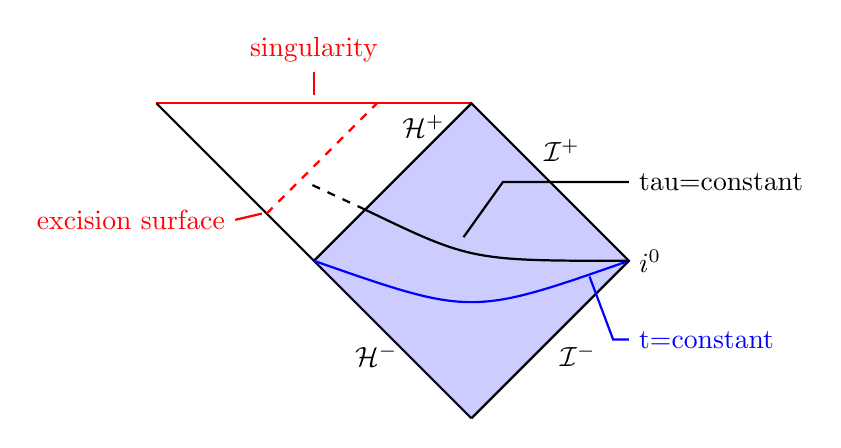
\begin{tikzpicture}

  \def\L{2.}

  % causal diamond
  \draw[thick,red] (-\L,\L) coordinate(stl) -- (\L,\L) coordinate (str);
  \draw[thick,black] (\L,-\L) coordinate (sbr)
    -- (0,0) coordinate (bif) -- (stl);
  \draw[thick,black,fill=blue, fill opacity=0.2,text opacity=1]
    (bif) -- (str) -- (2*\L,0) node[right] (io) {$i^0$} -- (sbr);

  % null labels
  \draw[black] (1.4*\L,0.7*\L) node[right]  (scrip) {$\mathcal{I}^+$}
               (1.5*\L,-0.6*\L) node[right] (scrip) {$\mathcal{I}^-$}
               (0.2*\L,-0.6*\L) node[right] (scrip) {$\mathcal{H}^-$}
               (0.5*\L,0.85*\L) node[right] (scrip) {$\mathcal{H}^+$};

  % singularity label
  \draw[thick,red] (0,1.05*\L)
    -- (0,1.2*\L) node[above] {singularity};
  % Scwharzschild surface
  \draw[thick,blue] (bif) .. controls (1.*\L,-0.35*\L) .. (2*\L,0);
  \draw[thick,blue] (1.75*\L,-0.1*\L)  -- (1.9*\L,-0.5*\L)
    -- (2*\L,-0.5*\L) node[right]
    {t=constant};
  % excision surface
  \draw[thick,dashed,red] (-0.3*\L,0.3*\L) -- (0.4*\L,\L);
  \draw[thick,red] (-0.33*\L,0.3*\L)
    -- (-0.5*\L,0.26*\L) node[left] {excision surface};
  % Kerr-Schild surface
  \draw[thick] (0.325*\L,0.325*\L) .. controls (\L,0) .. (2*\L,0);
  \draw[dashed,thick] (0.325*\L,0.325*\L) -- (-0.051*\L,0.5*\L);
  % Kerr-Schild label
  \draw[thick] (0.95*\L,0.15*\L) -- (1.2*\L,0.5*\L)
    -- (2*\L,0.5*\L) node[right] {tau=constant};
\end{tikzpicture}
